\documentclass{article}

\usepackage{graphicx}
\usepackage{tikz}
\usepackage{tikzsymbols}
\usetikzlibrary{calc,patterns,shapes.geometric}
\pagestyle{empty}
\usepackage[margin=0pt]{geometry}
\geometry{papersize={14in,12in}}

\def\centerarc[#1](#2)(#3:#4:#5){\draw[#1] ($(#2)+({#5*cos(#3)},{#5*sin(#3)})$) arc (#3:#4:#5);}

\begin{document}
	\begin{figure}
		\centering
		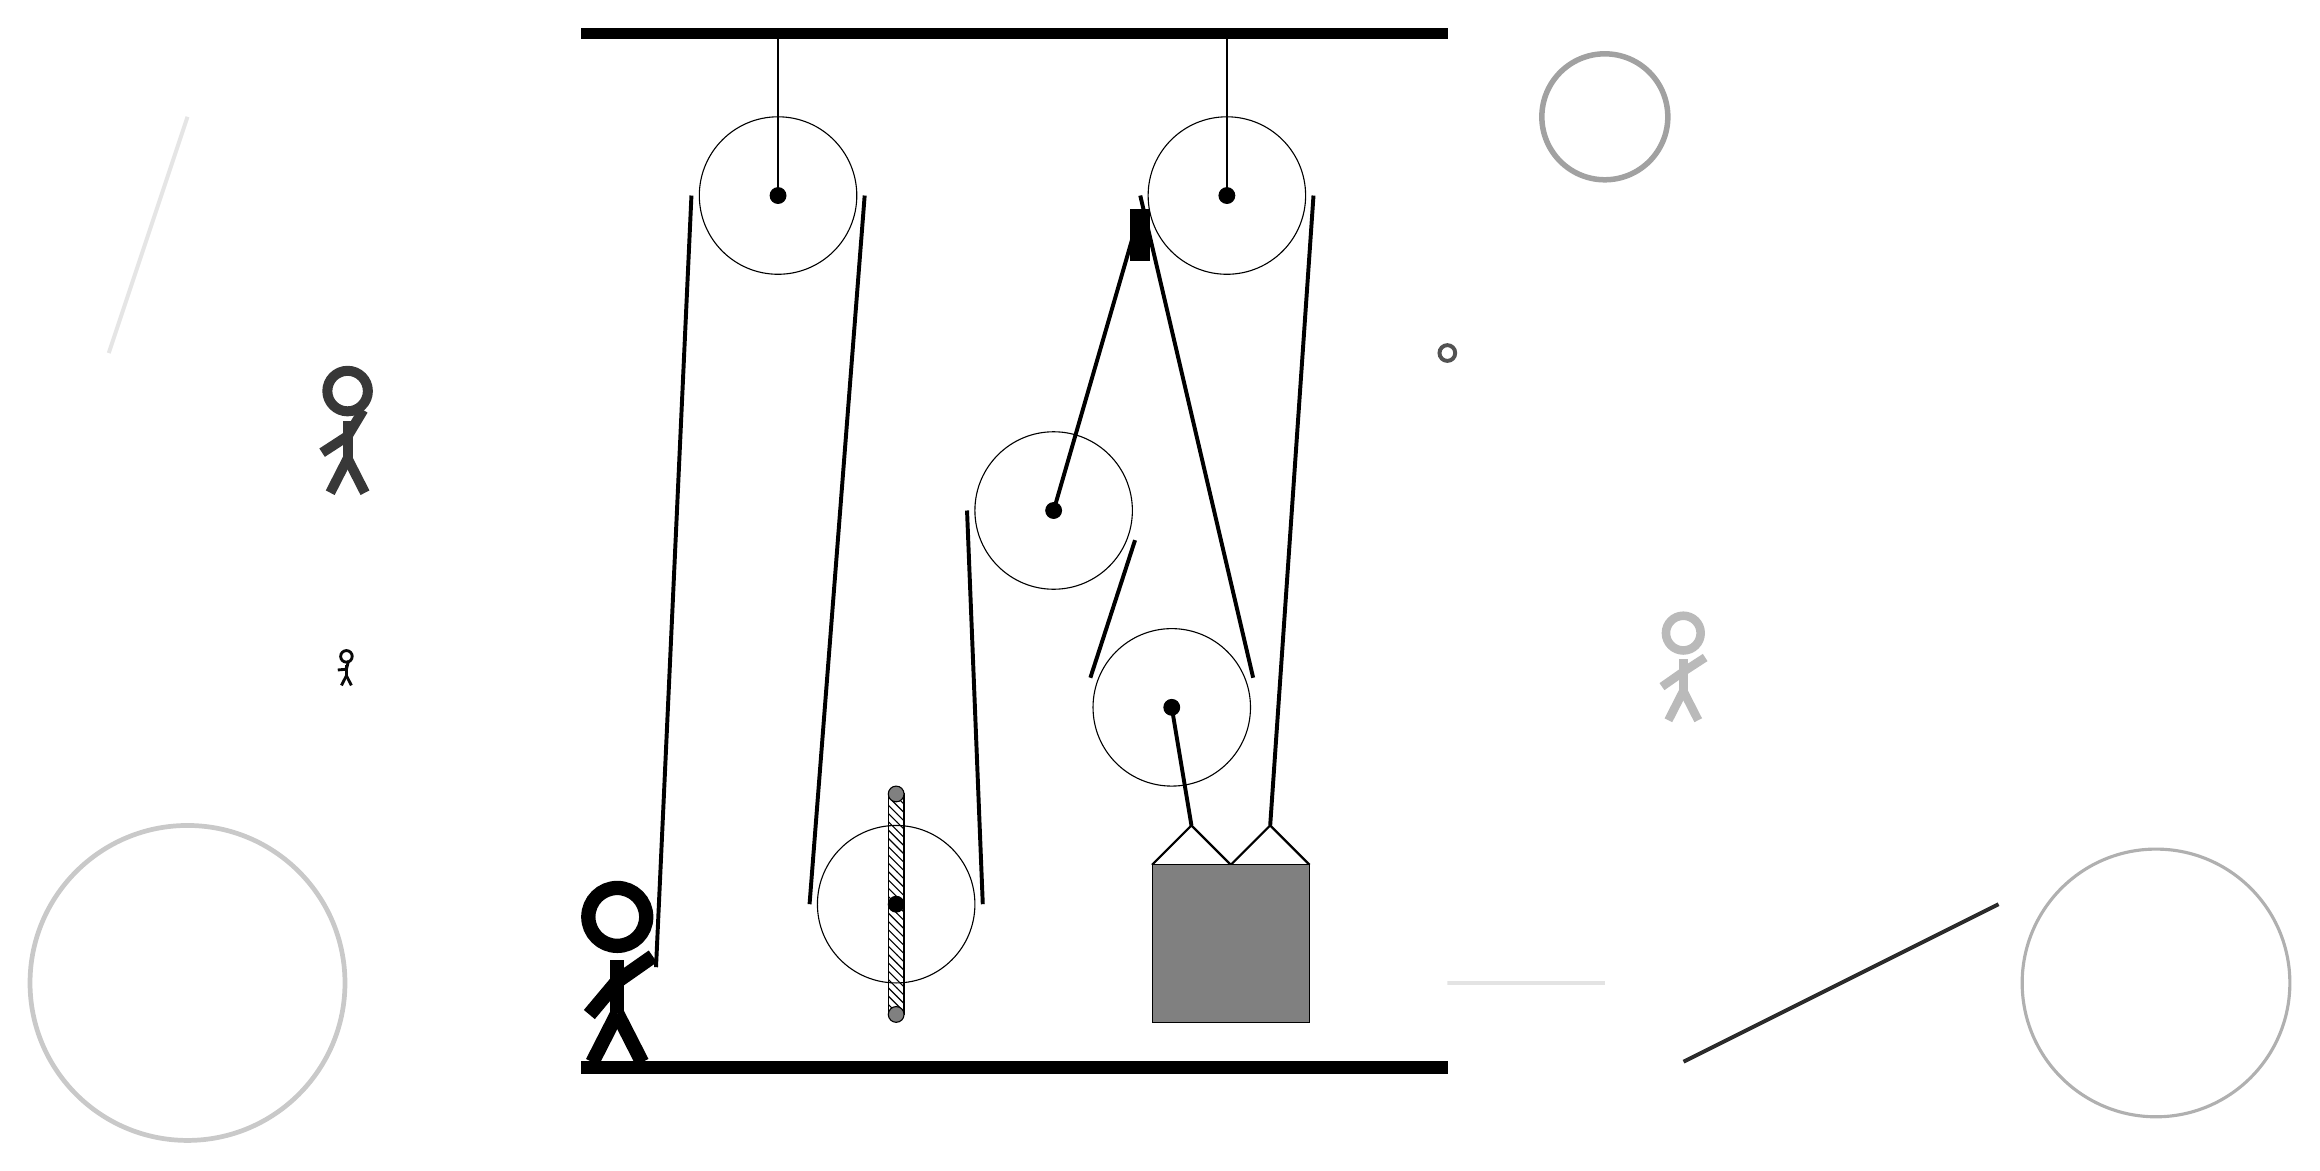
\begin{tikzpicture}
			%%%%% START %%%%%
			
			\draw[fill=black] (-6, 10) rectangle (5, 10.125);
			
			\draw (0, 4.0) circle (1);
			\draw[fill=black] (0, 4.0) circle (0.1);
			
			\draw (1.5, 1.5) circle (1);
			\draw[fill=black] (1.5, 1.5) circle (0.1);
			
			\draw (2.2, 8.0) circle (1);
			\draw[fill=black] (2.2, 8.0) circle (0.1);
			\draw[thick] (2.2, 8.0) -- (2.2, 10);
			
			\draw (-3.5, 8.0) circle (1);
			\draw[fill=black] (-3.5, 8.0) circle (0.1);
			\draw[thick] (-3.5, 8.0) -- (-3.5, 10);
			
			\draw [line width=0.7mm, color=black!37](7, 9) circle (0.8);
			
			\draw [line width=0.5mm, color=black!68](5, 6) circle (0.1);
			\node[line width=0.4mm, color=black!27] at (8, 2) {\Strichmaxerl[6][35][33]};
			\node[line width=0.2mm, color=black!78] at (-9, 5) {\Strichmaxerl[7][33][59]};
			\draw[line width=0.5mm, color=black!10](-11, 9) -- (-12, 6);
			\draw[line width=0.4mm, color=black!11] (5, -2) rectangle (7, -2);
			
			\node[line width=0.4mm, color=black!97] at (-9, 2) {\Strichmaxerl[2][5][76]};
			
			\draw [line width=0.4mm, color=black!31](14, -2) circle (1.7);
			\draw[line width=0.5mm, color=black!83](8, -3) -- (12, -1);
			\draw [line width=0.6mm, color=black!21](-11, -2) circle (2.0);
			
			
			\draw (-2, -1.0) circle (1);
			\draw[fill=black] (-2, -1.0) circle (0.1);
			\draw[pattern=north west lines, pattern color=black] (-2.1, 0.4) rectangle (-1.9, -2.4);
			\draw[fill=black!50] (-2, 0.4) circle (0.1);
			\draw[fill=black!50] (-2, -2.4) circle (0.1);
			
			\draw[thick]  (1.25, -0.5) -- (1.75, 0.0) -- (2.25, -0.5) -- (2.75, 0.0) -- (3.25, -0.5);
			\draw[fill=black!50] (1.25, -0.5) rectangle (3.25, -2.5);
			\draw[line width=0.5mm] (-5.05, -1.8) -- (-4.6, 8.0);
			\centerarc[line width=0.5mm](-3.5, 8.0)(0:180:1.1);
			\draw[line width=0.5mm] (-2.4, 8.0) -- (-3.1, -1.0);
			\centerarc[line width=0.5mm](-2, -1.0)(180:360:1.1);
			\draw[line width=0.5mm] (-0.9, -1.0) -- (-1.1, 4.0);
			\draw[line width=0.5mm] (0, 4.0) -- (1.1, 7.8);
			\draw[line width=0.5mm, fill=black](1.0, 7.2) rectangle (1.2, 7.8);
			\centerarc[line width=0.5mm](0, 4.0)(-20:180:1.1);
			\draw[line width=0.5mm] (1.0337, 3.6238) -- (0.4663, 1.8762);
			
			\centerarc[line width=0.5mm](1.5, 1.5)(160:380:1.1);
			\draw[line width=0.5mm] (2.5337, 1.8762) -- (1.1, 8.0);
			\draw[line width=0.5mm](1.5, 1.5) -- (1.75, 0.0);
			\centerarc[line width=0.5mm](2.2, 8.0)(0:180:1.1);
			\draw[line width=0.5mm] (3.3, 8.0) -- (2.75, 0.0);
			
			\node at (-5.5, -1.9) {\Strichmaxerl[10][50][35]};
			
			\draw[fill=black] (-6, -3) rectangle (5, -3.15);
			
			%%%%% END %%%%%
		\end{tikzpicture}
	\end{figure}	
\end{document}